\section{Wire Connectivity Tests}
\label{sec:TheTest}

The main goal of the ICARUS TPC's connectivity tests here described has been to check the condition of the wires of the each anode plane of the detector; i.e., to look/check for wires not properly working or even disconnected. \\

The tests, as described in \cref{ssec:stand_chimn}, were done using a test box that sends a pulse of specific voltage, triggers the oscilloscope and receives back an output signal from the wires and sends it to oscilloscope where we can look and measure the expected peak and amplitude.\\

Since horizontal cables can't get a pulse injected, there was a slightly different procedure to test the 8 non-standard chimneys (See \cref{ssec:nonStd_chimn}). 


\subsection{Test box}
\label{ssec:TestBox}

The SLAC test box (Fig.) was designated specially for the ICARUS TPC wire plane connectivity tests. It's a portable battery powered device with dimensions $20\times 15\times 10$ cm.\\

\begin{figure}[htb]
\centering
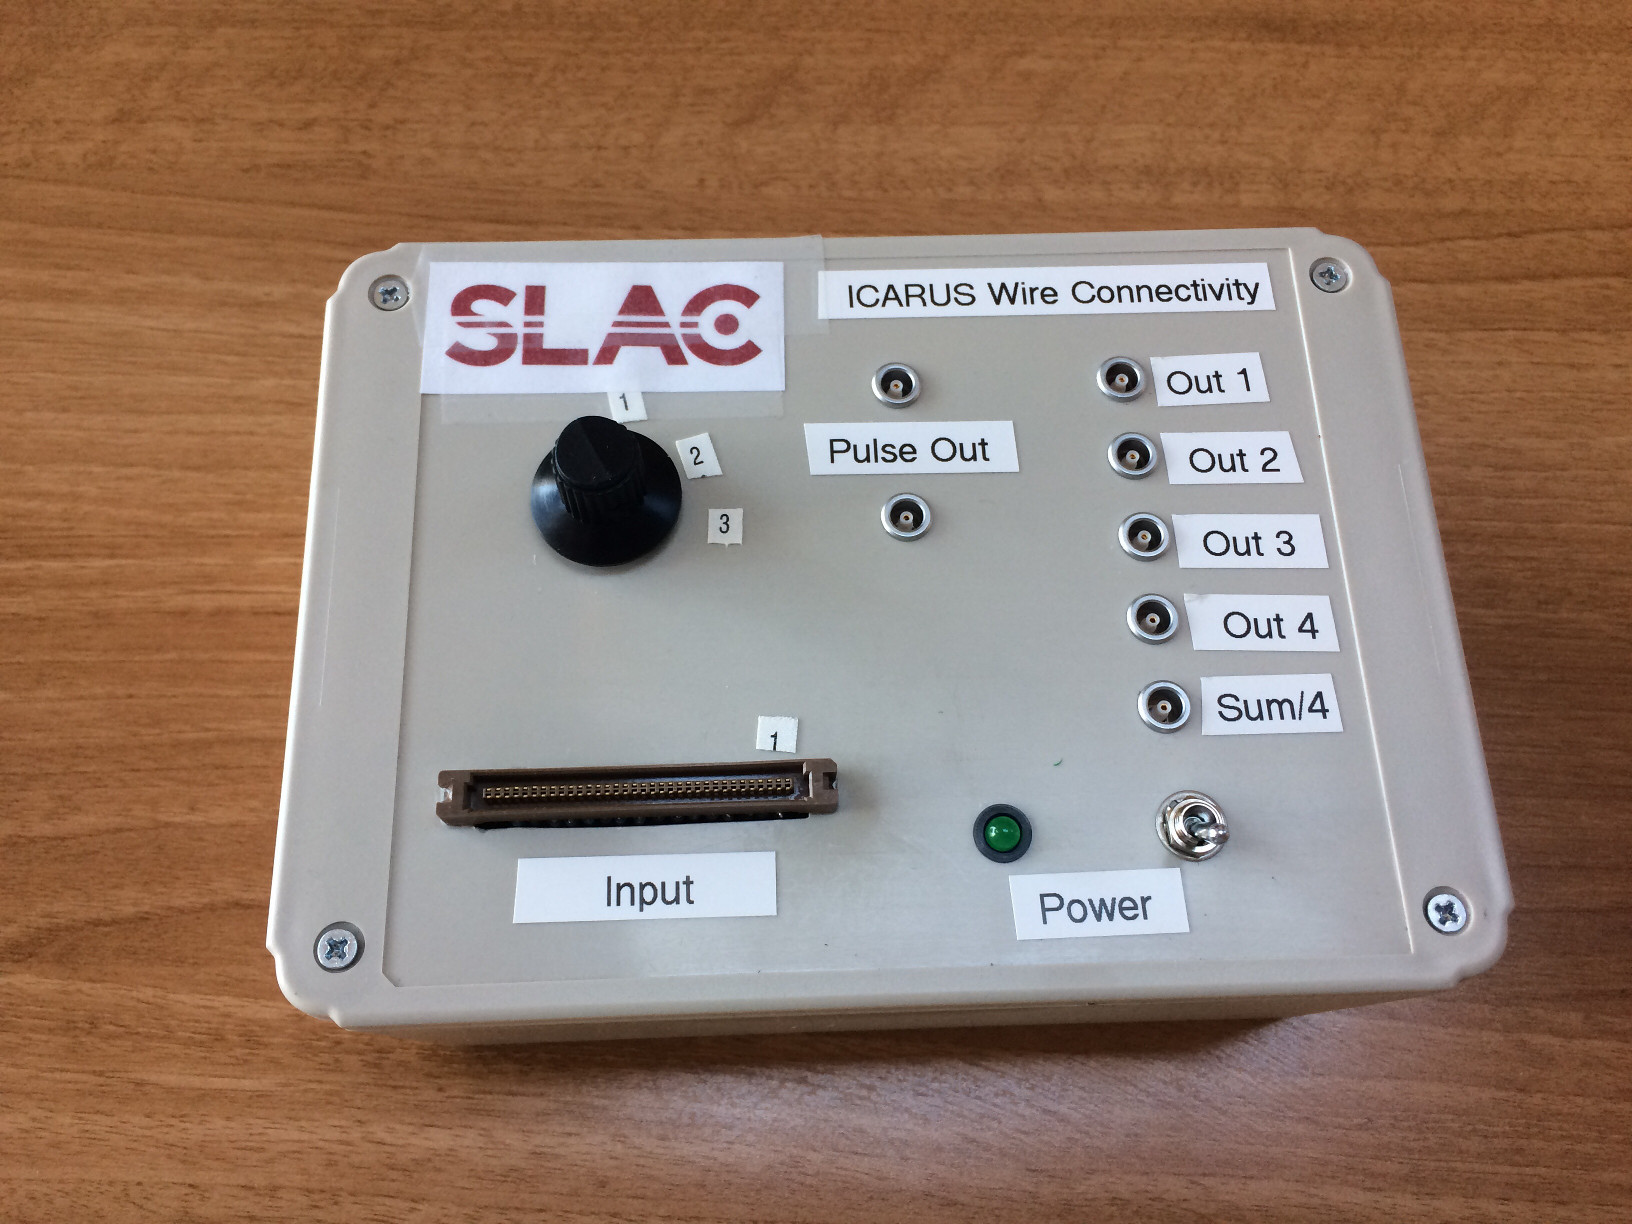
\includegraphics[width=0.8\linewidth]{fig/box1}
\caption{SLAC test box version 1}
\end{figure}

On the lid it contains:
\begin{itemize}
\item Built in pulser outputs on LEMO with both polarities,
\item Connector for a single flat ribbon of twisted-pairs cable: TPC cables plug into this connector with all grounds connected together.
\item An 8-position rotary switch that switches all 4 channels at a time,
\item The test pulse: $100$ Hz, $5$ V, $1 \mu $s rise time, $100 \mu $s length.

Two test boxes were built. It was found out that the cable shields, although connected together, were not grounded in the box. This was observed as a full size signal of about $1.5$ V.  The second version of the box contains extra outputs that allowed us to ground the shields of the connectors (Fig. second box). 
\end{itemize}

%SPEND MORE WORDS (regarding schematics of the electronics inside) ON THE TEST BOX!!!!



\subsection{Standard Chimneys}
\label{ssec:stand_chimn}

%The standard chimneys of the detector are the 2 to 19 $1$m tall cylinders that are bolted to the flanges on top of the cryostats (Fig.).

%\begin{figure}[H]
%\centering
%\includegraphics[scale=0.1]{fig/chimn}
%\caption{Chimneys installed, view from south to north.}
%\end{figure}

The TPC cables were pulled out from the detector through all the chimneys (Fig.) and the tests were performed in the following way: \\


%THIS PARAGRAH/INFO goes in Part II.
%The standard chimneys contain $18$ flat ribbon connectors each, $8$ pulser cables, groups of cables that belongs to the photomultipliers (High Voltage and signal) and optical fibers.\\

%\begin{figure}[H]
%\centering
%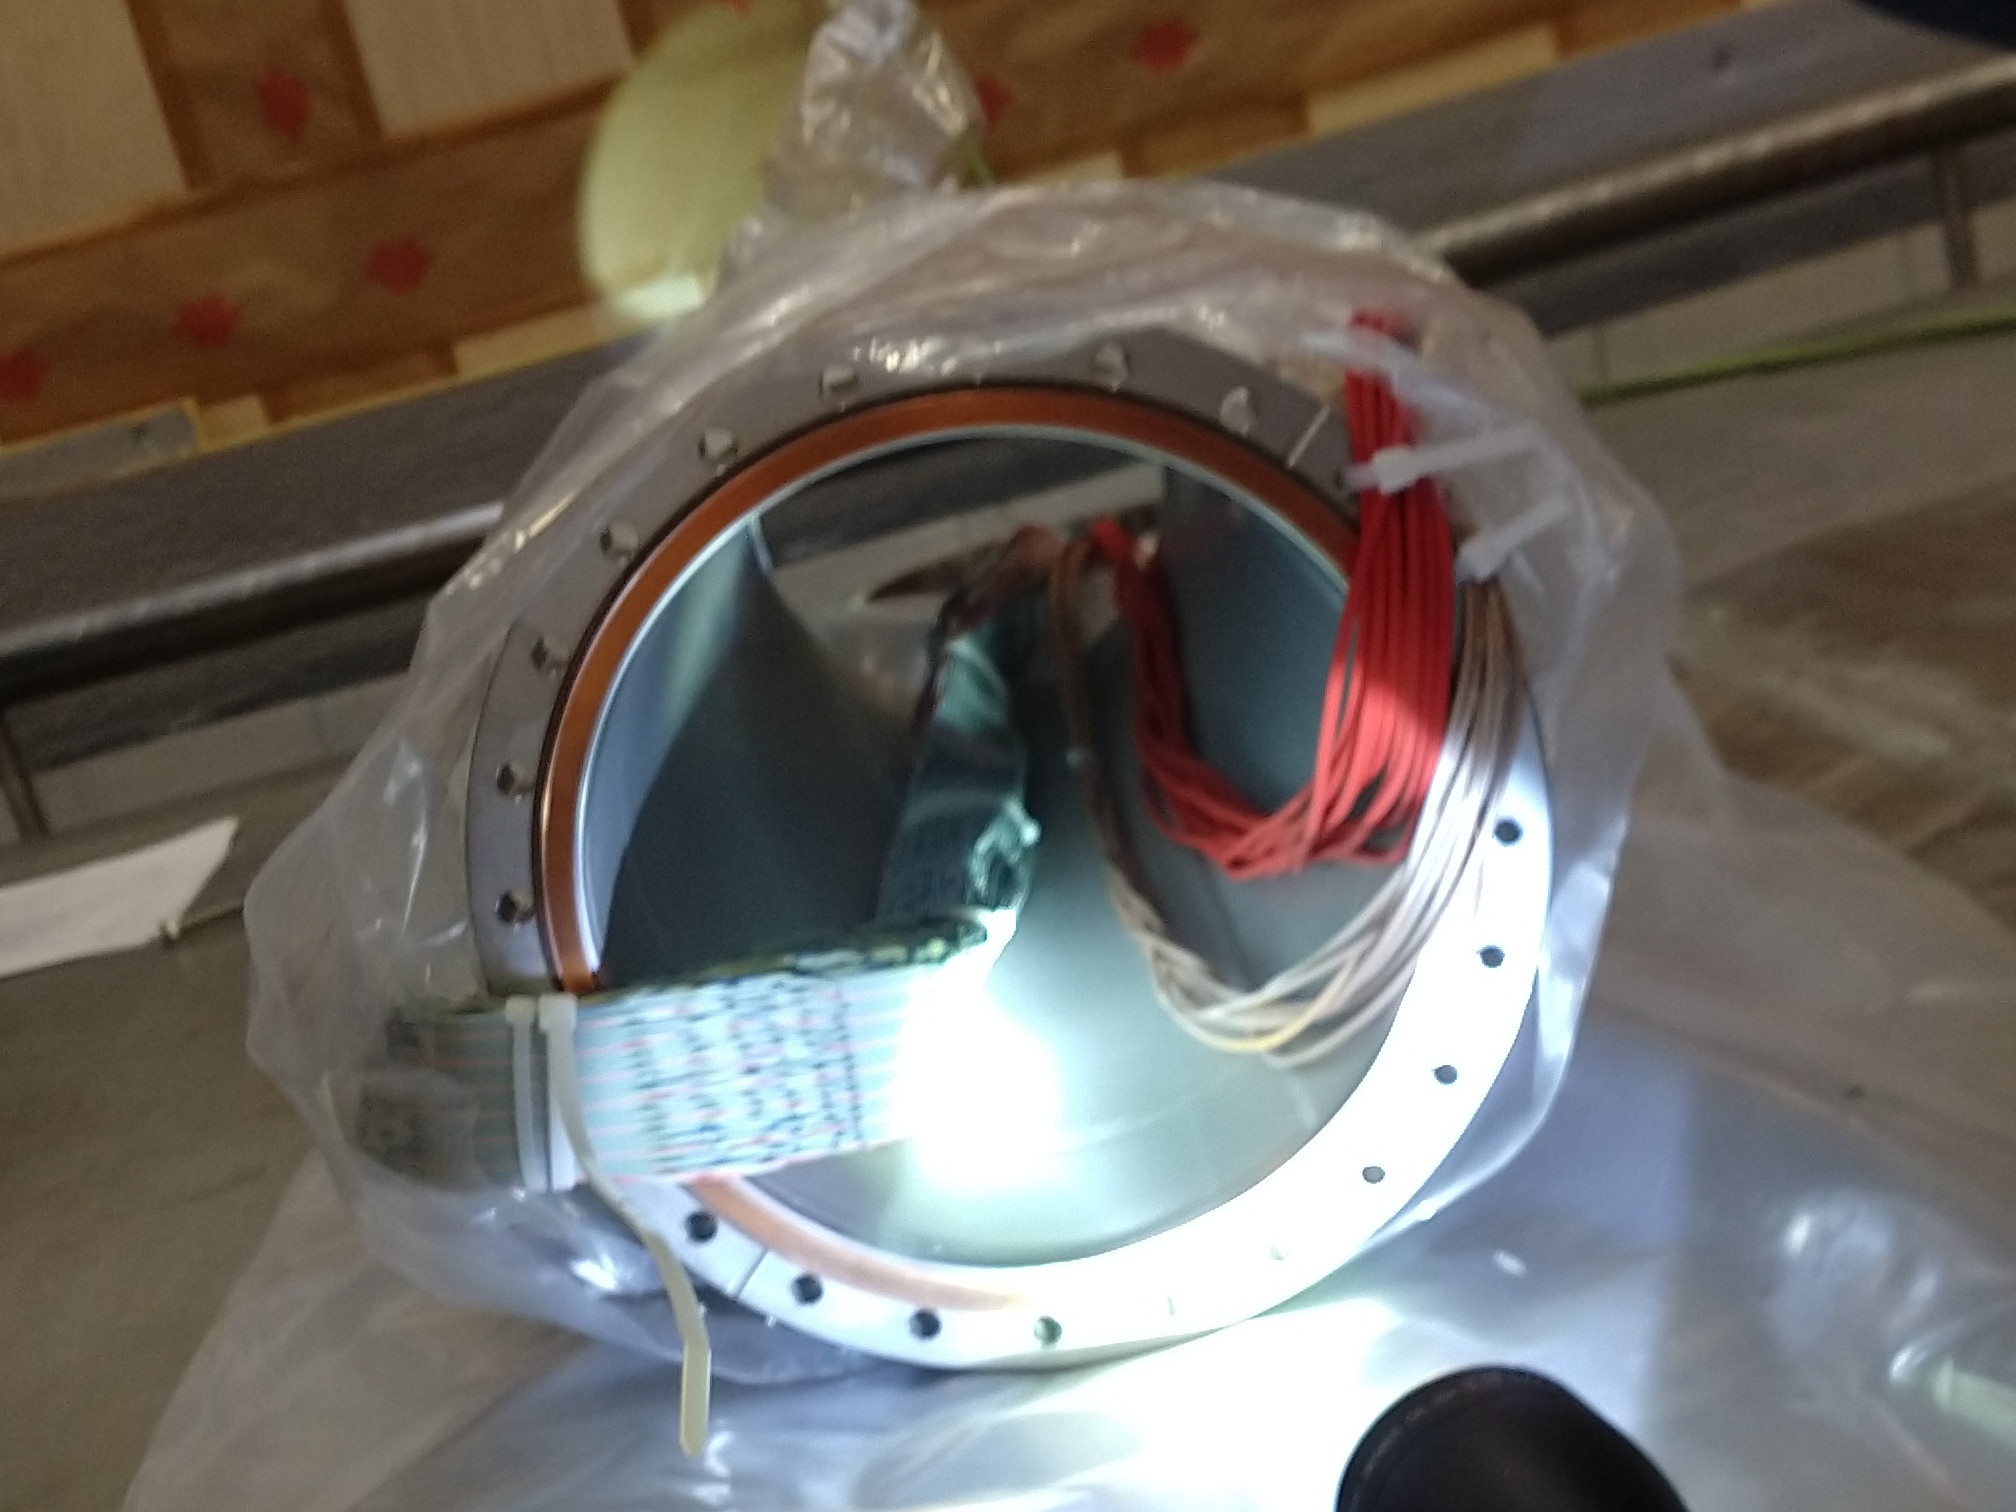
\includegraphics[scale=0.06]{fig/cab1} 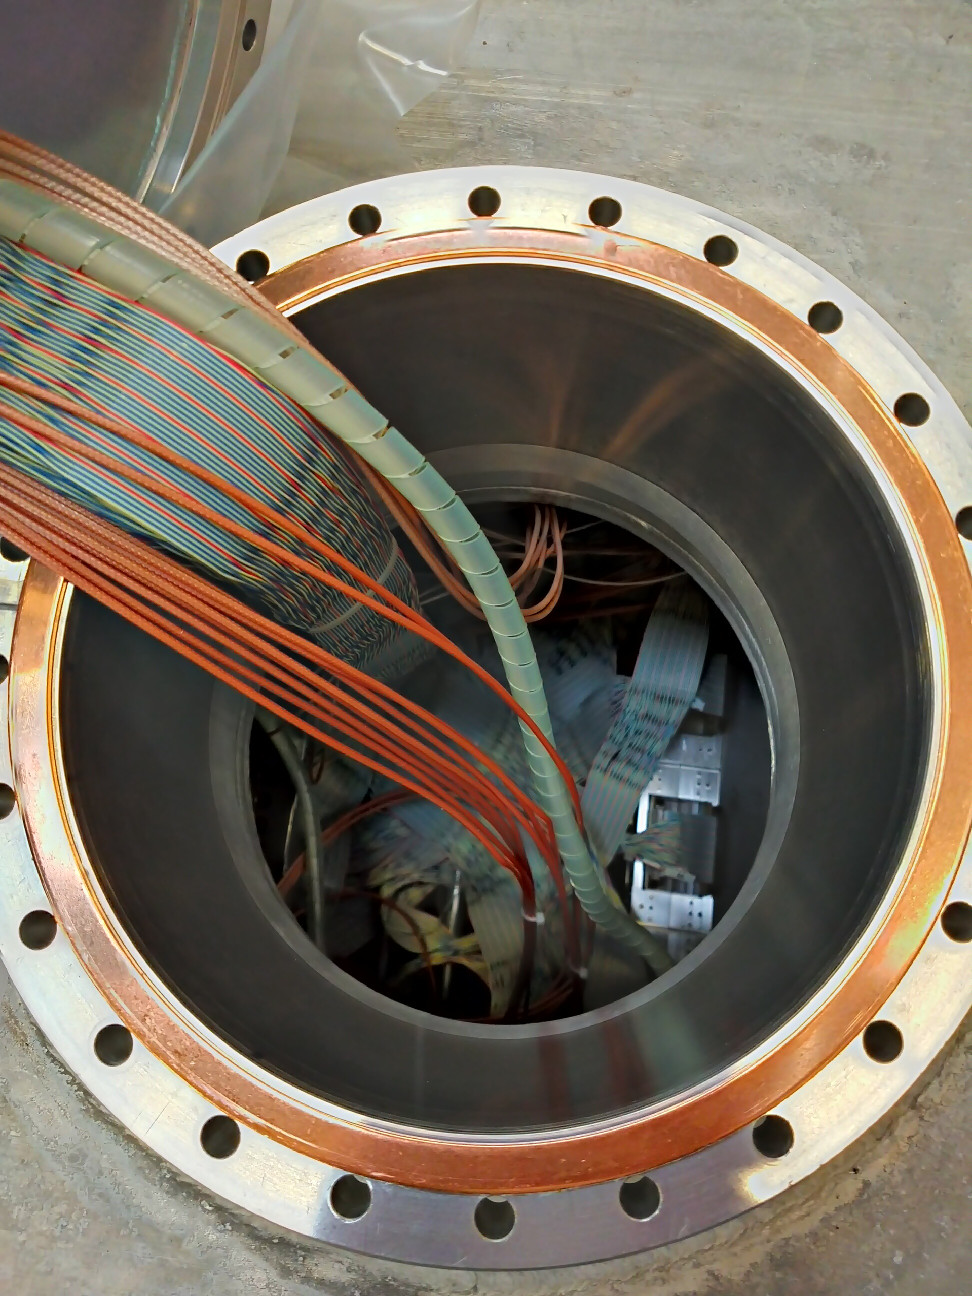
\includegraphics[scale=0.08]{fig/cab2}
%\caption{Left: Installation of a chimney. Right: HV PMT's cables (red), TPC connectors (colored flat ribbon cables)}
%\end{figure}


%Also this lines go in Part II
%The cables of interest are:
 
%\begin{itemize}
%\item 4 of the 8 SMA cables, the ones with red tag,

%\begin{figure}[H]
%\centering
%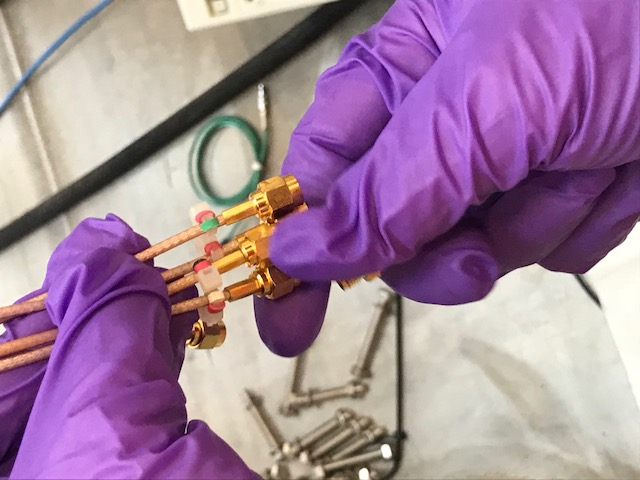
\includegraphics[scale=0.3]{fig/SMA} 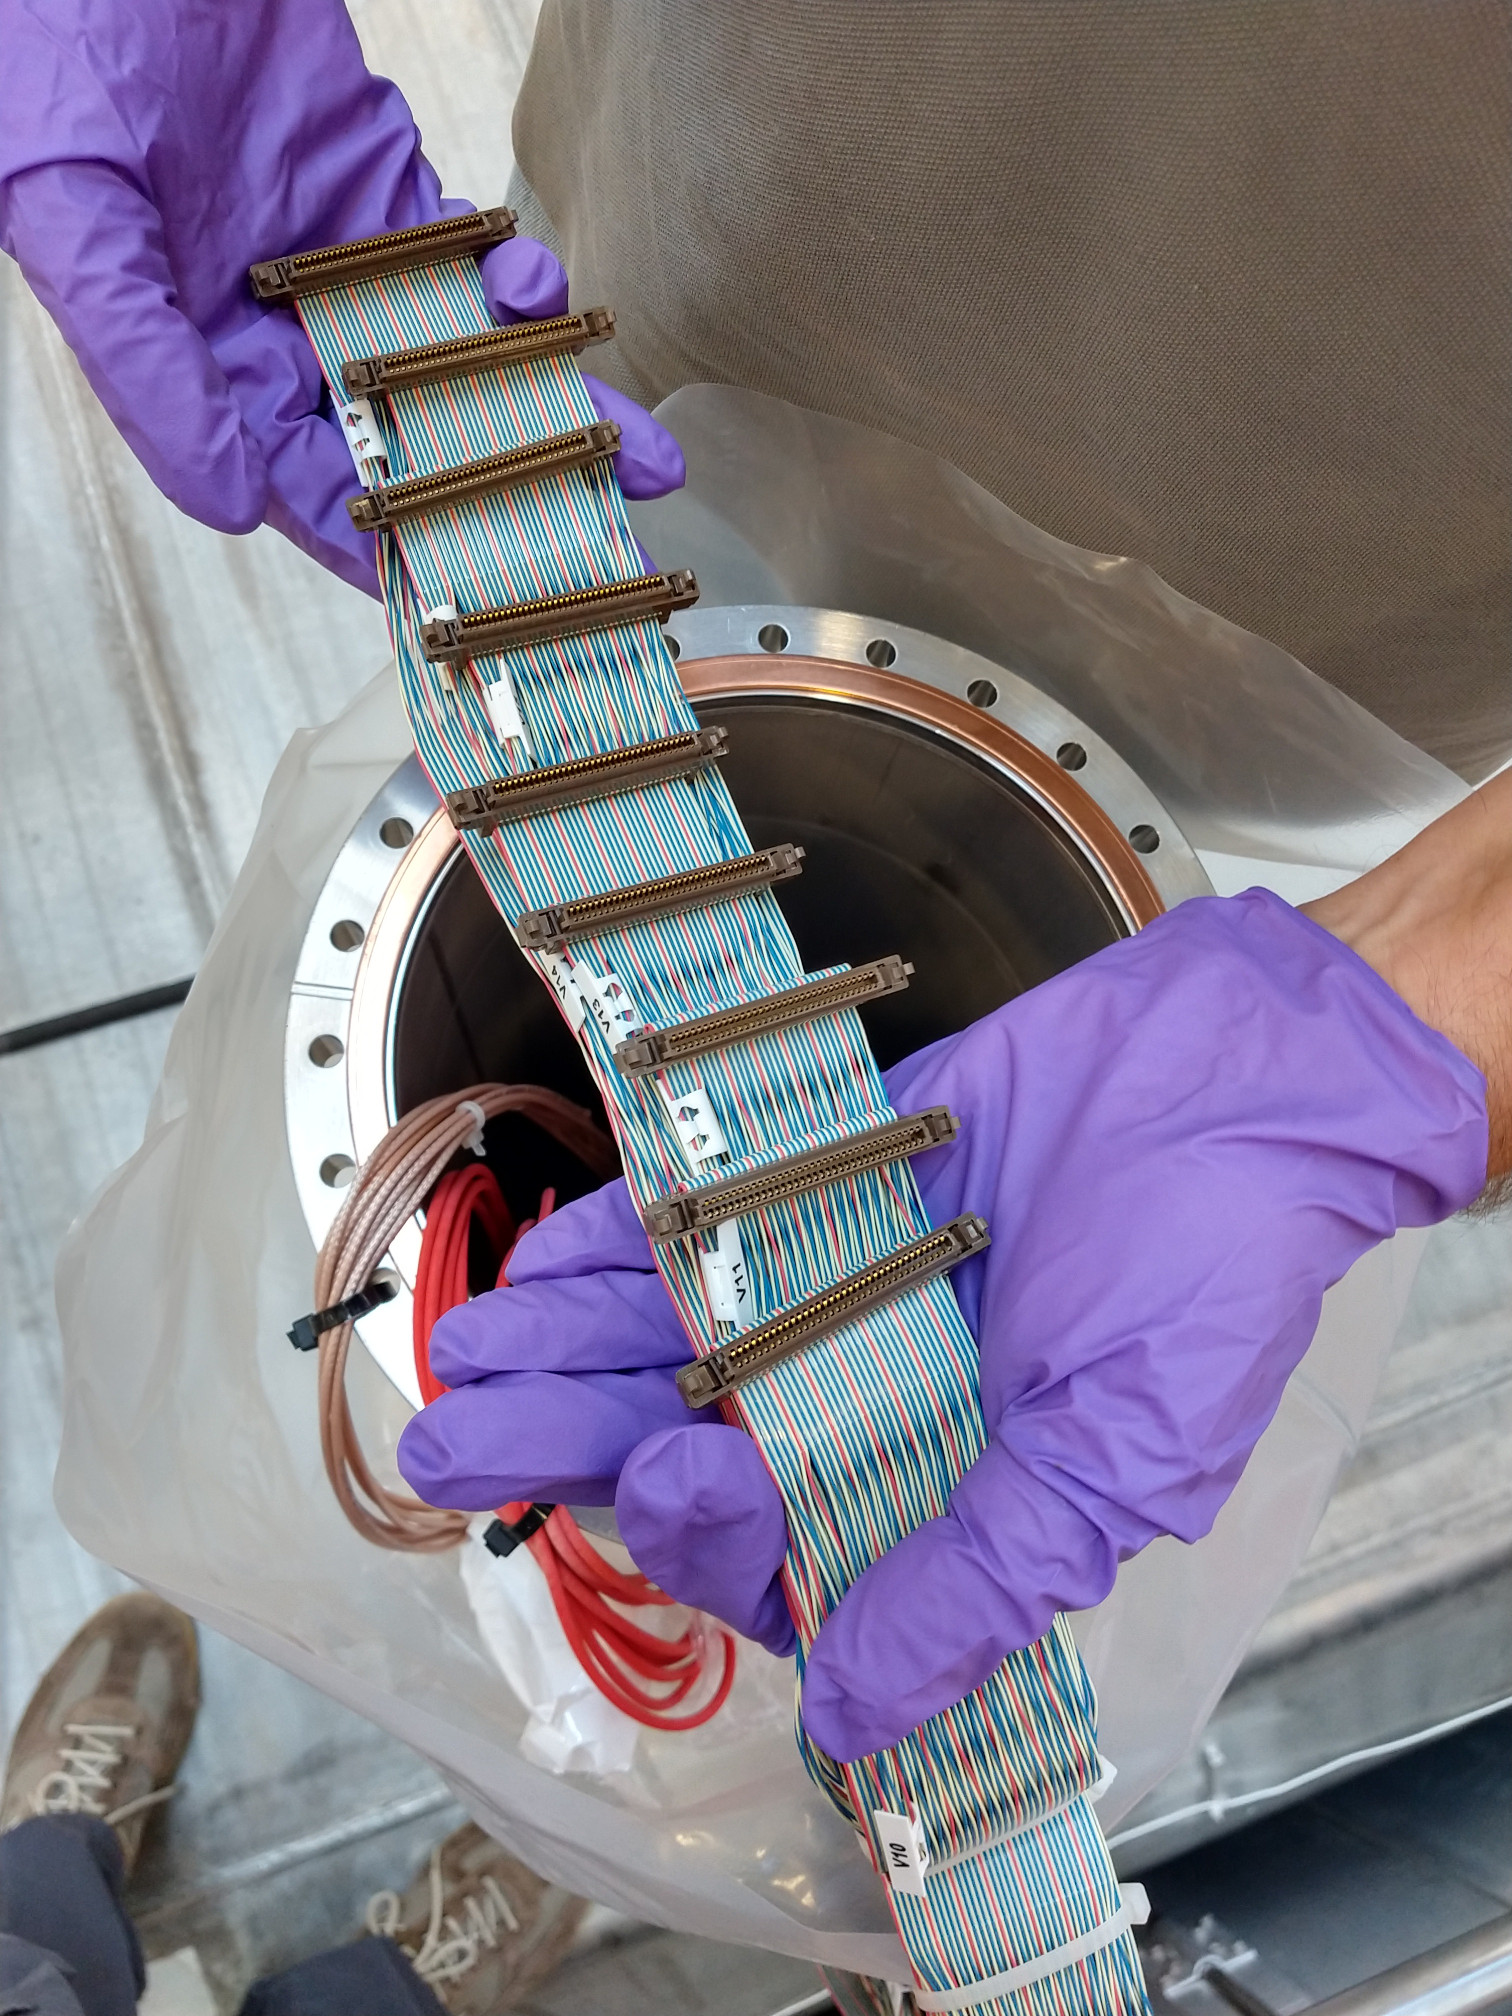
\includegraphics[scale=0.05]{fig/conn1}
%\caption{Left: SMA pulser cables, Right: 32 TPC wires per each single flat ribbon of twisted-pairs cables.}
%\end{figure}

%\item the $18$ flat ribbon connectors.

%\end{itemize}

\textit{Procedure:}\\
\begin{enumerate}
\item The external trigger was connected from one of the test-pulse output of the box to the oscilloscope (at the back). Therefore, the setting for the trigger in the oscilloscope input was changed to: "EXT" (external).

\item 4 LEMO cables connected from the box to the four inputs of the oscillope correspond to four channels of the signal (Fig.).

\item A SMA-female coaxial cable goes connected on the "pulse-out" of the box via LEMO conection and the SMA-female side is connected to the pulser from the detector.

An important requirement before starting to take data was to test all 4 SMA cables (red tag) in the search for the highest pulse.

In order to verify that everything was working properly, the box was tested in-site by connecting the test-pulse output directly to one channel of the oscilloscope, with the settings changed to DC and $1$ M$\Omega $ and looked for the $5$ V square signal on the screen. In addition, we verified the SMA (from the detector) to LEMO (pulser cable from the box) connection by using a chain of LEMO to SMA-female plus SMA-male to LEMO to connect the test box to the oscilloscope.

\item For a systematic test, we chose to start from the cable S/V18 to S/V1. Since the test box injects and receives output signal from only 4 cables of a single flat ribbon connector, we had to swith through 8 positions with the black know on top of the box in order to test all 32 wires from 1 connector at a time. 

\item The waveforms seen on the screen of the oscilloscope were downloaded using a Python script written by S. Castells [ref] and stored in an external disk for an offsite analysis. 


\begin{figure}[H]
\centering
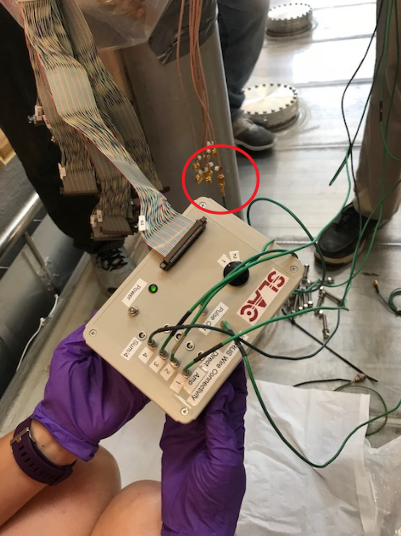
\includegraphics[scale=0.6]{fig/setup}
\caption{Set up of the hardware components. The red circle shows the SMA to LEMO connectors through which the box injects the test pulse.}
\end{figure}




\end{enumerate}




\subsection{Non-standard chimneys}
\label{ssec:nonStd_chimn}

The non-standard chimneys are the 8 corners of both cryostats, see Fig. Apart from the difference in size between standard and non-standard chimneys, the latter ones contain the horizontal and corner wire connectors. \\

As described on \cref{sec:Detector} the configuration of the horizontal wires does not allow to inject a pulse directly to the wires and therefore a different way to test them was developed. \\
The test pulse was injected to 32 wires of Induction-2 plane at once. From one standard chimney, two or three chimneys away from the corner, a connector between 2 and 9 was choosen and plugged in to a board (<-name?). To pulse those 32 wires we use the same conexion from the test box: a chain LEMO to SMA cables and to one of the 4 red-tagged pulser cables from the chimney.  

% -----------------------------------------------------------------------------
\subsection{Data acquisition}
\label{ssec:DAQ}

The test box output was monitored and sampled via
\href{https://www.tek.com/datasheet/digital-phosphor-oscilloscopes-0}{Tektronix
TDS 3054C oscilloscope}. This oscilloscope can digitise and send out the
input signals, providing \(10^4\) samples per channel. The data
acquisition code, written by Sergi Castells, reads a sequence of
waveforms from each oscilloscope channel. Each waveform is stored in its
own comma-separated value file (CSV), with a resolution is of 0.1 µs for
the time and 10 mV for the signal amplitude. Therefore the waveform
samples span 1 millisecond, and they are at baseline by roughly 60-80\%
of the time.

The testing procedure included cycling across all 8 switch positions of
the test box for each connection, and recording 10 waveforms for each of
the 4 channels monitored in the selected position. For each switch
position, therefore, 40 waveforms are recorded. The total data size as
stored in the final form is about 500 MiB per chimney.

% -----------------------------------------------------------------------------
\subsection{Data sets}
\label{ssec:data-sets}

The original acquisition software by Sergi Castells grants the operator
some options that affect the name of the waveform files. An
acquisition-driving code was developed that reduces those options and
enforces a file name pattern:

\begin{verbatim}
waveform_CH<channel>_CHIMNEY_<chimney>_CONN_<connector>_POS_<position>_<index>.csv
\end{verbatim}

where:

\begin{itemize}
\tightlist
\item
  \texttt{\textless{}channel\textgreater{}} is the \emph{oscilloscope
  channel} the waveform is read from, which ranges from \texttt{1} to
  \texttt{4}
\item
  \texttt{\textless{}chimney\textgreater{}} is in the form
  \texttt{\textless{}module\textgreater{}\textless{}row\textgreater{}\textless{}index\textgreater{}},
  with both module and row denoted by geographical position as
  \texttt{E} (east) or \texttt{W} (west), and the chimney number being
  between \texttt{01} and \texttt{20}; for example, \texttt{WE07}
\item
  \texttt{\textless{}connector\textgreater{}} is the name of the
  connector plugged in the test box, made of a letter (\texttt{S} or
  \texttt{V}) and the zero-padded connection number in the range from
  \texttt{01} to \texttt{18}, e.g. \texttt{V05}.
\item
  \texttt{\textless{}position\textgreater{}} is the setting of the test
  box switch selecting four channels among the 32 on the connector; it
  ranges from \texttt{1} to \texttt{8}
\item
  \texttt{\textless{}index\textgreater{}} is a waveform counter;
  following Sergi's convention, this is a sequential number unique
  within waveforms on the same connector and oscilloscope channel.
  Assuming that 10 waveforms are taken per channel, position
  \texttt{POS\_1} will have indices from \texttt{1} to \texttt{10},
  \texttt{POS\_2} from \texttt{11} to \texttt{20}, and so on, up to
  \texttt{POS\_8} with indices \texttt{71} to \texttt{80}.
\end{itemize}

320 waveform files are expected per connector (10 waveforms for each of
32 channels, split in 4 oscilloscope channels and 8 test box switch
positions), and 5760 per chimney. These files are stored in separate
directories, one per chimney. The name of the directory follows the same
convention as above, that is:

\begin{itemize}
\tightlist
\item
  \texttt{CHIMNEY\_\textless{}chimney\textgreater{}} in the form
  \texttt{\textless{}module\textgreater{}\textless{}row\textgreater{}\textless{}index\textgreater{}},
  with both module and row denoted by geographical position as
  \texttt{E} (east) or \texttt{W} (west), and the chimney number being
  between \texttt{01} and \texttt{20}; for example,
  \texttt{CHIMNEY\_WE07}
\end{itemize}

The whole dataset taken in the test session of August 2018 is currently
stored in Fermilab dCache at the path:

\begin{verbatim}
/pnfs/icarus/persistent/commissioning/connectivity/201808
\end{verbatim}

The script \texttt{checkChimneyFiles.sh} (currently stored in
\texttt{/icarus/data/commissioning/connectivityTest/201808/scripts})
checks the presence of all the expected files for each chimney
directory.

% -----------------------------------------------------------------------------
\subsection{Data format}
\label{ssec:data-format}

Each waveform is stored in its own comma-separated value file (CSV). The
file name follows the pattern described above. Each line in the file
corresponding to a sample, totaling 10000 lines for each waveform. Each
sample is described by values in floating point text representation,
with scientific notation: time in seconds, and signal level in volt. For
example:

\begin{verbatim}
0.0,2.08
1e-07,2.08
2e-07,2.12
[...]
\end{verbatim}

No metadata is saved in the file. This data format can be easily read
directly by ROOT \texttt{TGraph}.

% -----------------------------------------------------------------------------
\subsection{Streamlined interactive data acquisition}
\label{ssec:streamlined-interactive-data-acquisition}

The original code by Sergi Castells required the operator to change
parameters on the command line on each acquisition, plus an additional
step at the end of the test each connector, that is to reset a counter
stored in a text file.

After a few interactions with this approach, we wrote additional
software (\emph{test driver}) automating most of the steps required from
the operator. This enforced a specific procedure both for testing and
for software setup.

The procedure comprises testing one chimney at a time, and proceeding
from connection 18 (\texttt{V18} or \texttt{S18}) down to 1
(\texttt{V01} or \texttt{S01}), and on each connector test the channel
switching the test box to the position from 1 to 8 in strict sequence.
The whole sequence must be strictly followed.

The test diver is unfortunately hard to correctly set up the first time.
The software is all written in python 2, and it requires both the python
Visual Instrument Software Architecture (PyVISA, exposing the module
\texttt{visa}) and CERN ROOT (PyROOT, exposing the module \texttt{ROOT})
interfaces. It proved hard to get to a configuration where python would
load both at the same time on OSX, while no Linux laptop was tried. The
pattern that seemed more likely to succeed was to install PyVISA
following online instructions found at
\texttt{https://pyvisa.readthedocs.io/en/master/index.html}, which
included installing National Instrument backend software {[}1{]}, which
we used in its release 18.0. After having tested that the \texttt{visa}
module correctly work, again as described in the linked documentation,
we compiled ROOT (6.14) from source \emph{in the same environment} (that
is , in the same shell).

The setup of the test instrumentation is the same as for the software
from Sergi. The data acquisition session is run within a single
\texttt{python} session. Its setup includes importing the test driver
module (\texttt{testDriver.py}), setting the IP address of the
oscilloscope in use, and finally instantiate the test driver. A possible
setup sequence is:

\begin{verbatim}
from testDriver import *
loadScopeReader('192.168.230.29')
reader = ChimneyReader()
\end{verbatim}

After this per-session setup, the data acquisition is driven by choosing
the chimney (e.g. \texttt{reader.start("EW09")}) and repeatedly call the
acquisition function (\texttt{reader.next()}). It is also possible to
skip to remove the last acquisition and repeat it, or skip to a
different one.

{[}1{]} Registration to National Instruments web site is required in
order to download the software, but no fee payment was required to
download the driver package.
